\chapter{Tools, patterns and firsts decisions}

Nowadays we can build almost any kind of software with a lot of differents
language from which to choose, but as if that were not enough there
are also a lot of architectures that are possible to follow, and beside
of this it will necesary choose where deploy our software, or how
doc it, or how magane our work team, etc. A lot of options that it
will necesary to choose and that can make the difference between the
success or failure of our project. So, what about of these decisions
in this project? Take a look about it.
fld fsldf dsk

\section{Architecture}

Almost any kind software or tool can be builded of differents ways, independetly
of this behaviour or the goals that it must achieve. Some ways are more specific
to achieve some specific behaviour and anothers.

\subsection{Kind of software}
Based of informal requirements was thinked that the best option must be a \textbf{web app} for a lot of reasons. First of all because is the simplest way to offer an app that can run in almost any device (with a \textit{simple\footnote{Actually a browser is one of the more complex pieces of software, but here is labeled as simple because is a software that the mayority of device like smartphones, tablet, etc, have by default and for the most non technical people isn't a complex software, nothing could be further from the truth.}} browser).

\subsection{Why microservices?}

When we think in an app, of any type, the most of time we think in a software
running in a single machine, with more or less hardware availabe, where all
related with the software are inside of the same machine.

Now, we hearing all the time about microservices, that are in synthesys the
oposite of the traditional monolithic clasical apporach in software architecture,
and seem like if your design are not based in this mean you are outdated or your
design is fdirectly wrong.
Well, this is not totally true but neither false. The goal of this section is
not describe the advantages and drawbacks of this approach, but yes justify why
is their choise.

Microservices are actually a variant of SOA (Service-Oriented Architecture) ,
that simplifying a lot is architecture of a software system composed of two
different systems, working together to do the service which the software was design.

TODO: poner bien.
Dr. Peter Rodgers introduced the term "Micro-Web-Services" during a presentation at Cloud Computing Expo in 2005

TODO: reparar de la wikipedia
Microservices is a specialization of an implementation approach for service-oriented architectures (SOA) used to build flexible, independently deployable software systems.[21] The microservices approach is a first realisation of SOA that followed the introduction of DevOps and is becoming more popular for building continuously deployed systems.[22]

TODO: Ver como poner las citas en Latex
This brings us to the canonical definition of microservices, from Lewis/Fowler:

In short, the microservice architectural style is an approach to developing a
single application as a suite of small services, each running in its own process
and communicating with lightweight mechanisms, often an HTTP resource API.
These services are built around business capabilities and independently deployable
by fully automated deployment machinery. There is a bare minimum of centralised management
of these services, which may be written in different programming languages and
use different data storage technologies.

Service-oriented architecture (SOA) was first described by Gartner in 1996
(see SSA Research Note SPA-401-068 , 12 April 1996, "'Service Oriented'
Architectures, Part 1" and SSA Research Note SPA-401-069 , 12 April 1996,
"'Service Oriented' Architectures, Part 2"),

TODO Poner referencia a Gartner


Much more that the trend in the develop of apps, all of change of
paradigm inspired in distributed system, now over http and focussed
(especially) in web apps as a consequence of the multiple benefits
to this kind of sofwate. \bigskip

Language agnostic, scalable, size ajustables, independently, the system
splited in litle pieces with this boundaries ...

\subsection{Why polyglot database?}

With the mircroservices approach the system will be some very differents
database to do some diferents things. So, in general we can see our
backend like a black box when the data persists in a polyglot database.
That means that the data is save in differents ways, using diferetns
formats and diferents driver to manage this. There are a group of
data that it need saved with certain relations, due to its nature,
so a relational database seem perfect to do this, but this kind of
databases (like MySQL) can been slowly or too heavy for other tasks
of kind of processes, like data analysis.

\section{Code strategy}


Entire project will be stored in a single repository, using git as control
versions system.

\subsection{Version Control System}

Git\footnote{Git is a free and open source, distributed version control system
created by Linus Torvalds} is the perfect tool to achieve maintain a more o
less easy workflow between developers minimizing the risks, and the huge list of
plugins to different software and IDEs do this perfect to work, dismissing another
as Subversion, Mercurial, Fossil, or Bazzar.

The reason to use a single repository is because the mechanism to maintain the
consistency between projects are not enough easily to do the develop agile.
In spite of, git offers us a lot of tools that can improve enormouslly our
workflow, as for example the Git Submodules\footnote{Submodules allow you to keep a
Git repository as a subdirectory of another Git repository.
This lets you clone another repository into your project and keep your commits
separate.} or Git Hooks\footnote{Git has a way to fire off custom scripts when
certain important actions occur. There are two groups of these hooks:
client-side and server-side. Client-side hooks are triggered by operations such
as committing and merging, while server-side hooks run on network operations
such as receiving pushed commits} between another.

\subsection{Hub}

For other hand we have to do another choice, select the remote hub of our repositories
or Git repository hosting service. The most popular since some years has been GitHub,
is a web-based Git or version control repository and Internet hosting service.
It offers all of the distributed version control and source code management (SCM)
functionality of Git as well as adding its own features,
launched at 2008
but there are another options as Bitbucket\footnote{web-based hosting service
that is owned by Atlassian, used for source code and development projects that
use either Mercurial (since launch) or Git
launhed at 2008},
SourceForge\footnote{another system launched at 1999} and specially
GitLab\footnote{launched at 2011, was written by Dmitriy Zaporozhets and Valery
Sizov from Ukraine. The code is written in Ruby. Later, some parts have been
rewritten in Go.} (with a big grow ultimately).


\subsection{Develop workflow}

Another of the mainly problem easy to find in the develop when are involved
few people is the organization of the contribution of a repo, but if the project
is composed of few subprojects this can be worst. For this reason was choise the
strategy to have a only repo with subfolders.
So, taked this decision remains to be defined how will work the repo in the
diferent phases or the develop.

To do this we will follow the standar, using branchs to develop features and
maintain a good state of the versioning of project.

So, as we can see in the picture, we are going to use \textit{develop} branch
to do the develop, where we are going to work in minimal changes and will do
a fork when we want to do some representative change in the code, as new functionality or
some big correction.


\begin{center}
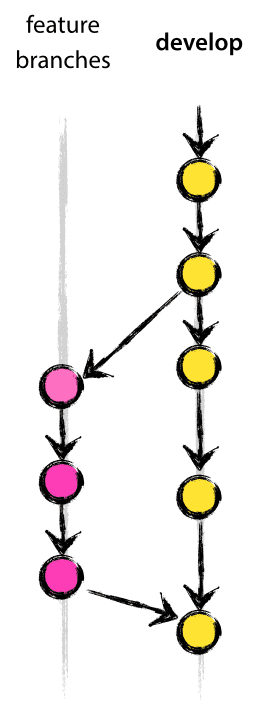
\includegraphics[scale=0.25]{img/git/feature_branches.png}
\end{center}

For other hand when the all code to launch a final release we will fork the
repo in a \textit{release} branch to while the team continue with the develop
in the mainly develop branch ot in a issue form of this another part of the
team (or itself, is the same), will prepare the code to production, taking a look
because there are some bug, fix it and when all are testend an correctly working
put the project in exactly this verison in master (doing a merte) and this is
when officially a new version of program will be launched.

\begin{center}
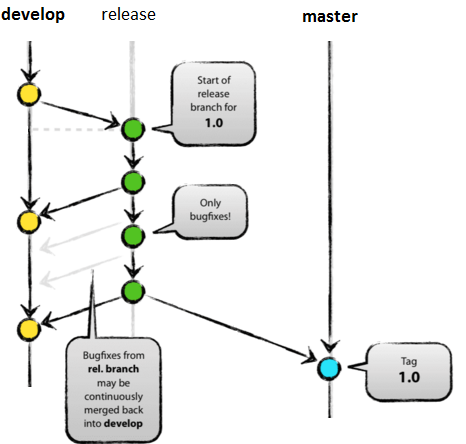
\includegraphics[scale=0.4]{img/git/release_branches.png}
\end{center}

There are some variations of this standard workflow but for this kind of project
is perfect.

\section{Languages and frameworks}

As has been said before, almost any kind of software can be builded at infinite
ways, and this start with what language can do this. This means it could be
builded with Java, Ptyhon, C++, Go, Ruby, JavaScript, PHP,  (only talking about
backend) and with another list to frontend, in this deep list of possibilities,
we choose the most flexible and powerfull of all of them, Python and JavaScript.

Python because is one of hte most simplest and powerfull languages nowadays, and
JavaScript because is all an standard in the industry. Obviously the choise is
based also in the fact of both languages are really supported of community, have a
good learning curve and a lot of projects and systems are based in them.

JavaScript has been selected becuase Angular is writte in it. AngularJS is the
most powerfull framework nowdays to buil fas, clean and powerfull web apps.


\subsection{Communications}

\subsubsection{Data serialization format}


To exchange data between service we need to select a idiom which the services
will talk, which them will exhange information. That's mean mainly select how
will transform the objects anda data structures that servicres manage to be able
sender across the net.
We have some data serialization solutions, some very popular and another most
specific of very focused domains. So, the most commons are Json, Yaml,
Bson and ultimately MessagePack.

Each have their owns benefits and drawbacks but the selection has been easy, JSON.

\textbf{XML} (Extensible Markup Language), is a markup language, defined v1.0 by
W3C\footnote{World Wide Web Consortium, founder by Tim Berners-Lee at 1994 at MIT
(Massachusetts Institute of Technology) the consortium is made up of member
organizations which maintain full-time staff for the purpose of working together
in the development of standards for the World Wide Web.}

This is an example:
\begin{lstlisting}[language=xml,frame=none,numbers=none]
  <exam>
    <result>5.8</result>
    <type>Partial</type>
    <subject>Science</subject>
    <date>17-06-2018</date>
  </exam>
\end{lstlisting}

\textbf{JSON} JavaScript Object Notation, is an open-standard file format that uses
human-readable text to transmit data objects consisting of attribute–value pairs
Douglas Crockford originally specified the JSON format in the early 2000s;
two competing standards, RFC\footnote{ Request for Comments, is a type of
publication from the Internet Engineering Task Force (IETF) and the Internet
Society (ISOC), the principal technical development and standards-setting bodies
for the Internet. were invented by Steve Crocker in 1969 to help record
unofficial notes on the development of ARPANET} 7159 and ECMA\footnote{Ecma is a
standards organization for information and communication systems founded in 1961
to standardize computer systems in Europe.}-404, defined it in 2013.
The ECMA standard describes only the allowed syntax, whereas the RFC covers some
 security and interoperability considerations.

In spite of A restricted profile of JSON, known as I-JSON (short for "Internet JSON"),
defined in RFC 7493, is not as popular as original.

This is an example:
\begin{lstlisting}[frame=none,numbers=none]
  {
    "title": "The Picture of Dorian Gray",
    "author": "Oscar Wilde",
    "date": "July 1890"
  }
\end{lstlisting}


\textbf{YAML} (Yet Another Markup Language)
 is commonly used for configuration files, but could be used in transmision also,
 YAML 1.2 is a superset of JSON, whitch Latest release1.2 (Third Edition) was published
 at (1 October 2009; 7 years ago), YAML was first proposed by Clark Evans in 2001.

\begin{lstlisting}[frame=none,numbers=none]
  ---
  invoice: 34843
  date   : 2001-01-23
\end{lstlisting}


\textbf{BSON}
Binary JSON, is a computer data interchange format used mainly as a data storage
and network transfer format in the MongoDB database.
MongoDB represents JSON documents in binary-encoded format called BSON behind
the scenes. BSON extends the JSON model to provide additional data types,
ordered fields, and to be efficient for encoding and decoding within different languages.

\textbf{MessagePack}
byte array
is an efficient binary serialization format, like JSON but faster and smaller.

\begin{lstlisting}[frame=none,numbers=none]
{"compact": true, "schema": 0}
27Bytes

82 A7 compact C3 A6 schema 00
18bytes
\end{lstlisting}

And another aprox as zerorp, It builds on top of ZeroMQ and MessagePack

\subsubsection{Protocol}

APIRest

Wikipedia
Representational state transfer (REST) or RESTful Web services are one way of providing interoperability between computer systems on the Internet. REST-compliant Web services allow requesting systems to access and manipulate textual representations of Web resources using a uniform and predefined set of stateless operations. Other forms of Web service exist, which expose their own arbitrary sets of operations such as WSDL and SOAP.[1]

RPC

In distributed computing, a remote procedure call (RPC) is when a computer program causes a procedure (subroutine) to execute in another address space (commonly on another computer on a shared network), which is coded as if it were a normal (local) procedure call, without the programmer explicitly coding the details for the remote interaction.

  gRPC

gRPC is an open source remote procedure call (RPC) system initially developed at Google. It uses HTTP/2 for transport, Protocol Buffers as the interface description language, and provides features such as authentication, bidirectional streaming and flow control, blocking or nonblocking bindings, and cancellation and timeouts. It generates cross-platform client and server bindings for many languages.

We will talk a bit more about this in the Develop chapter.


\subsection{Testing}

The tool that we will use for any testing involved in the backend of the project
will be PyTest. Launched at 2004 by Holger Krenel is one of the most complete
suites for testing over Python.
Is really easy to use and allow do some things that is very difficult with another
frameworks as built-in \textit{unittest} python package, somethings as the use of
fixtures of or the amount of plugint that it has.

Focused on the problem it will be used to make all unittest of the core of services,
libraries and auxiliary programs and testing the entire functionality of the service
when it has a role of black box.


\subsection{Documentation}

As is saided the tool Sphinx is used to build the doc of the service.
That basically inspect the code files mixing this with all the files
that we write (pure doc) to show this as a web based documetnation
(easy to read and understand).

\section{Storage}

With the storage occurs exactly the same, there are a huge list of options to
choose. The fast answer in the most of cases is: Why do not use a relational
database, as MySQL for example? If wer are thinking in a little system maybe a
good choice, always that we data model is adjuste to this kind of system. But
every people  knows the deficients and a the complexity of develop with system
with this database. Mainly the performance when we are talking a bout million
of arrays of object stored. So, as we are talking before, our goal in this project
is work with a lot of data, which a part are pure relational and another can be
processed of another way.

If you have a logic data model like as this project have is not easy choise one
of all database engine to model this. SQL systems is very powerfull for some
things but not for another (or not simply) and object oriented databases is
really powerfull and simply to develop with it when the data haven't a lot of
relations (althouth can be modeled also).
so, why choise one between them? Why do not both? This is the approach selected,
build a system with a Polyglot Database, that means: much better select the better
engine for any kind of data instead of try to use the same for all.
And this approach joined with microservices architecture give as the first
conceptually of our system, when each microservice of domain work with their
data, using for this their own database engine, their own kind of data, and
until their own language if is precise.


So, focused in this project, we are going to use mainly two systems, SQL
relational database system in a service (we will talk more about it after),
and a NoSQL service, in this case Google Datastore, a fast and lightweight
engine to mange a object oriented database.

At the moment of write this chapetr had been evaluated MongoDB as the best
choise, but the facilities of the platform selected (detailed after) was made
that the G. Datastore was selected finally. Beside of this if the project are
rebuild now have not dude, Mongo will be selected afte the experience ( the
reasons will be explained with more detail in the conclusion of the work).

\subsection{Versions}

Talking about Python has selected 2.7 version not for the best reasons.
And is because the sandbox of Google App Engine do not allow another upper versions.

About Angular the selectioni Angular1.x. Seem a bit old, the new version 2.x
is really popular now and the community is talking about the next two levels
uppper version AngularJS 4.x.
The selection of the lower version is simple, a lot of interesting material
about this, the most of problems that we can find already solved or with a lot
of help and the maintenance.

\subsection{Frameworks}

Flask

At the moment to write this work has been used it but exists another
that are been used in another project that have more potentia because have
better performance, as Falcon (betweern anothers).









\section{Platforms}

Google App Engine, Amazon Web Services, Microsoft Azure, IBM BlueMix,
Heroku, CloudFoundry, etc...

Realizar comparativa y justificar muy bien la eleccion.

\section{Documentation}



\subsubsection {ds}

\section{License}

GPL3 Free software
